% ============================================================
% Capítulo 1 — Fundamentos Históricos e Filosóficos
% OpenCode Ecosystem Core — Manual Universal
% ============================================================

\chapter{Fundamentos Históricos e Filosóficos dos Ecossistemas Cognitivos}

\begin{quote}
\textit{``A questão de se as máquinas podem pensar é tão relevante quanto a questão de se os submarinos podem nadar.''} \\
--- Edsger W. Dijkstra, 1984
\end{quote}

\section{Da Máquina de Turing à Era dos Large Language Models}

A história da inteligência artificial (IA) é, em essência, a história da tentativa humana de compreender e replicar os mecanismos do pensamento. Este percurso, que se estende por quase um século, pode ser organizado em ondas paradigmáticas que se sobrepõem e se complementam, cada uma deixando um legado arquitetural que o OpenCode Ecosystem Core herda e integra.

\subsection{O Problema da Decidibilidade e a Máquina Universal (1936--1950)}

Alan Turing estabeleceu as fundações teóricas da computação moderna em seu artigo seminal de 1936, ``On Computable Numbers, with an Application to the Entscheidungsproblem'' \cite{turing1936computable}. Neste trabalho, Turing introduziu o conceito de uma \textbf{máquina universal} --- um dispositivo abstrato capaz de simular qualquer outro dispositivo computacional, desde que programado adequadamente. A máquina de Turing é composta por:

\begin{enumerate}
    \item Uma \textbf{fita infinita} dividida em células, cada uma contendo um símbolo de um alfabeto finito;
    \item Uma \textbf{cabeça de leitura/escrita} que se move bidirecionalmente sobre a fita;
    \item Um \textbf{registro de estado} que armazena o estado atual da máquina;
    \item Uma \textbf{tabela de transição} (o ``programa'') que, dado o estado atual e o símbolo lido, determina o próximo estado, o símbolo a escrever e a direção do movimento.
\end{enumerate}

\begin{figure}[htbp]
\centering
\begin{tikzpicture}[node distance=2cm, auto]
    \node[draw, rectangle, minimum width=12cm, minimum height=1.5cm] (tape) at (0,0) {Fita infinita: \texttt{... | 0 | 1 | 1 | 0 | 1 | B | B | ...}};
    \node[draw, rectangle, minimum width=3cm, minimum height=2.5cm, above=0.5cm of tape] (head) {Cabeça Leitura/Escrita};
    \node[draw, rectangle, rounded corners, minimum width=4cm, minimum height=2.5cm, right=2cm of head] (control) {Controle Finito\\(Tabela de Transição)};
    \draw[->, thick] (head) -- (tape);
    \draw[<->, thick] (head) -- (control);
    \node[below=0.3cm of tape, font=\footnotesize] {Modelo da Máquina de Turing Universal (1936)};
\end{tikzpicture}
\caption{Arquitetura conceitual da Máquina de Turing Universal.}
\label{fig:turing_machine}
\end{figure}

A relevância deste modelo para o OpenCode Ecosystem Core é profunda: o \textbf{MetaBus} (Capítulo 9) atua como a ``fita infinita'' do ecossistema --- um barramento de eventos onde todos os agentes podem ler e escrever --- enquanto o \textbf{Orquestrador Central} funciona como a ``tabela de transição'' que decide qual agente deve ser ativado com base no estado atual do sistema.

Em 1950, Turing publicou ``Computing Machinery and Intelligence'' \cite{turing1950computing}, introduzindo o famoso \textbf{Teste de Turing} (originalmente chamado de ``The Imitation Game''). A pergunta fundamental --- ``Can machines think?'' --- inaugurou o campo da IA como disciplina científica. Turing propôs que, em vez de definir ``pensamento'', deveríamos avaliar se uma máquina pode se passar por um ser humano em uma conversa textual. Este critério comportamental --- julgar pela performance observável, não pela essência interna --- antecipa o princípio de \textbf{BehavioralGate} utilizado pelo Trust Engine do OpenCode (Capítulo 8): agentes são avaliados por seus resultados observáveis, não por suas intenções declaradas.

\subsection{A Conferência de Dartmouth e o Nascimento da IA (1956)}

No verão de 1956, John McCarthy, Marvin Minsky, Nathaniel Rochester e Claude Shannon organizaram a histórica \textbf{Dartmouth Summer Research Project on Artificial Intelligence} \cite{mccarthy1956dartmouth}. O proposal da conferência, redigido por McCarthy, cunhou o termo ``Artificial Intelligence'' e estabeleceu a premissa fundadora:

\begin{quote}
``The study is to proceed on the basis of the conjecture that every aspect of learning or any other feature of intelligence can in principle be so precisely described that a machine can be made to simulate it.''
\end{quote}

Este otimismo inicial --- acreditava-se que o problema da IA seria resolvido em um verão --- deu lugar a décadas de avanços e retrocessos. A conferência de Dartmouth produziu duas contribuições duradouras:

\begin{enumerate}
    \item \textbf{Logic Theorist} (Newell, Shaw \& Simon, 1956): considerado o primeiro programa de IA, capaz de provar teoremas matemáticos usando raciocínio simbólico heurístico \cite{newell1956logic}. Este trabalho lançou as bases do paradigma simbólico e introduziu o conceito de ``heurística'' --- regras práticas que guiam a busca em espaços de solução exponenciais.
    \item \textbf{Princípio da Resolução} (Robinson, 1965): um método completo para prova automática de teoremas em lógica de primeira ordem \cite{robinson1965machine}. Este princípio é utilizado pelo motor de raciocínio Z3 integrado ao OpenCode (\texttt{reasoning/engines.py}), demonstrando como técnicas da IA clássica permanecem relevantes.
\end{enumerate}

\subsection{Paradigma Simbólico: A Era de Ouro da IA Clássica (1956--1974)}

O paradigma simbólico, também conhecido como \textbf{GOFAI} (Good Old-Fashioned Artificial Intelligence), baseava-se na hipótese do \textbf{sistema de símbolos físicos} (Newell \& Simon, 1976) \cite{newell1976computer}:

\begin{quote}
``A physical symbol system has the necessary and sufficient means for general intelligent action.''
\end{quote}

Segundo esta hipótese, a inteligência emerge da manipulação de símbolos discretos segundo regras formais. Os sistemas especialistas dos anos 1970 e 1980 --- como MYCIN (diagnóstico médico), DENDRAL (análise química) e XCON (configuração de computadores) --- representam o ápice desta abordagem \cite{buchanan1984rule}.

\begin{table}[htbp]
\centering
\caption{Marcos do Paradigma Simbólico e sua Herança no OpenCode}
\label{tab:symbolic_legacy}
\begin{tabular}{p{3cm}p{4cm}p{4cm}p{3cm}}
\hline
\textbf{Sistema} & \textbf{Ano} & \textbf{Contribuição} & \textbf{Herança OpenCode} \\
\hline
Logic Theorist & 1956 & Primeiro provador de teoremas & Motor Z3 (SMT) \\
ELIZA & 1966 & Processamento de linguagem natural & Agente 25 (Linguística) \\
SHRDLU & 1970 & Compreensão de linguagem em mundos de blocos & Blackboard (espaço compartilhado) \\
MYCIN & 1976 & Sistema especialista com fatores de certeza & Confidence Ledger \\
R1/XCON & 1980 & Configuração automática (10.000+ regras) & Catálogo de 128+ agentes \\
Cyc & 1984 & Base de conhecimento de senso comum (ontologia) & Memória semântica MetaBus \\
\hline
\end{tabular}
\end{table}

O OpenCode Ecosystem Core preserva e transcende o paradigma simbólico através de múltiplos mecanismos:
\begin{itemize}
    \item O \textbf{Specification-Driven Development} (SDD) formaliza conhecimento em especificações estruturadas (\texttt{specs/*.md}), reminiscente das bases de conhecimento dos sistemas especialistas;
    \item O \textbf{Blackboard} (\texttt{mci/blackboard.py}) implementa um espaço de tuplas onde agentes especializados colaboram, herdeiro direto da arquitetura Hearsay-II para reconhecimento de fala;
    \item Os \textbf{motores de raciocínio} (\texttt{reasoning/engines.py}) oferecem Z3 (SMT), SymPy (álgebra simbólica), Kanren (programação lógica) e Critical (pensamento crítico).
\end{itemize}

\subsection{O Inverno da IA e a Ascensão Conexionista (1974--2012)}

O relatório Lighthill (1973) \cite{lighthill1973artificial} para o British Science Research Council criticou duramente a falta de progresso da IA, desencadeando o \textbf{Primeiro Inverno da IA} no Reino Unido. O relatório identificou a ``explosão combinatória'' como obstáculo fundamental: sistemas simbólicos não escalavam para problemas reais.

Paralelamente, o \textbf{paradigma conexionista} ressurgia. Embora McCulloch e Pitts (1943) \cite{mcculloch1943logical} tenham proposto o primeiro modelo matemático de neurônio artificial, e Rosenblatt (1958) \cite{rosenblatt1958perceptron} tenha demonstrado o Perceptron --- capaz de aprender a classificar padrões linearmente separáveis ---, o campo sofreu um golpe com o livro ``Perceptrons'' de Minsky e Papert (1969) \cite{minsky1969perceptrons}, que demonstrou as limitações dos perceptrons de camada única (incapazes de resolver o XOR).

\begin{figure}[htbp]
\centering
\begin{tikzpicture}[scale=0.9]
    % Perceptron simples
    \node[draw, circle] (x1) at (0,2) {$x_1$};
    \node[draw, circle] (x2) at (0,0) {$x_2$};
    \node[draw, circle] (bias) at (0,-2) {$1$ (bias)};
    \node[draw, circle, minimum size=1.5cm] (sigma) at (4,0) {$\Sigma$};
    \node[draw, rectangle, minimum width=1.5cm, minimum height=1cm] (act) at (7,0) {$f$};
    \node[right=1cm of act] (y) {$\hat{y}$};
    
    \draw[->] (x1) -- node[above] {$w_1$} (sigma);
    \draw[->] (x2) -- node[above] {$w_2$} (sigma);
    \draw[->] (bias) -- node[below] {$b$} (sigma);
    \draw[->] (sigma) -- node[above] {$z = \sum w_i x_i + b$} (act);
    \draw[->] (act) -- (y);
    
    \node[font=\footnotesize] at (0,-3) {Modelo do Perceptron (Rosenblatt, 1958)};
\end{tikzpicture}
\caption{Arquitetura do Perceptron. A função de ativação $f$ produz a saída binária.}
\label{fig:perceptron}
\end{figure}

O renascimento conexionista veio com o algoritmo de \textbf{backpropagation}, popularizado por Rumelhart, Hinton e Williams (1986) \cite{rumelhart1986learning}, que permitiu treinar redes neurais multicamadas. Três décadas depois, a convergência de três fatores --- big data, GPUs e arquiteturas profundas --- produziu a revolução do \textbf{Deep Learning}:

\begin{itemize}
    \item \textbf{AlexNet} (Krizhevsky, Sutskever \& Hinton, 2012) \cite{krizhevsky2012imagenet}: venceu o ImageNet com margem histórica, reduzindo o erro de 26\% para 15.3\%, demonstrando o poder das CNNs com GPUs;
    \item \textbf{Word2Vec} (Mikolov et al., 2013) \cite{mikolov2013efficient}: introduziu embeddings densos de palavras, capturando relações semânticas como $v_{\text{rei}} - v_{\text{homem}} + v_{\text{mulher}} \approx v_{\text{rainha}}$;
    \item \textbf{Seq2Seq com Atenção} (Bahdanau, Cho \& Bengio, 2015) \cite{bahdanau2015neural}: mecanismo de atenção que permite ao decoder ``focar'' em partes relevantes do input, precursor direto do Transformer.
\end{itemize}

\subsection{Paradigma Neuro-Simbólico: A Síntese}

O paradigma neuro-simbólico busca integrar o melhor dos dois mundos: a capacidade de aprendizado a partir de dados (conexionista) com o raciocínio lógico e a interpretabilidade (simbólico). Trabalhos seminais incluem:

\begin{itemize}
    \item \textbf{Neural Theorem Provers} (Rocktäschel \& Riedel, 2017) \cite{rocktaschel2017end}: unificação de redes neurais com backward chaining do Prolog;
    \item \textbf{DeepProbLog} (Manhaeve et al., 2018) \cite{manhaeve2018deepproblog}: integração de programação lógica probabilística com deep learning;
    \item \textbf{Graph Neural Networks} (Scarselli et al., 2009; Kipf \& Welling, 2017) \cite{kipf2017semi}: raciocínio relacional sobre grafos de conhecimento.
\end{itemize}

O OpenCode Ecosystem Core é intrinsecamente neuro-simbólico:
\begin{itemize}
    \item \textbf{Camada Transformer} (\texttt{transformer/}): processamento neural de linguagem natural e padrões;
    \item \textbf{Motores de Raciocínio} (\texttt{reasoning/}): lógica formal (Z3), álgebra simbólica (SymPy), programação lógica (Kanren);
    \item \textbf{MetaBus + Blackboard}: integração de ambos via barramento metacognitivo.
\end{itemize}

\subsection{Paradigma Metacognitivo: A Fronteira Atual}

O paradigma metacognitivo representa a convergência de três linhas de pesquisa:

\begin{enumerate}
    \item \textbf{Global Workspace Theory} (Baars, 1988; Dehaene \& Changeux, 2011) \cite{baars1988cognitive, dehaene2011experimental}: a consciência como um espaço de trabalho global onde informações competem por acesso e são broadcasted para módulos especializados;
    \item \textbf{Reflexion Framework} (Shinn et al., 2023) \cite{shinn2023reflexion}: agentes que aprendem com seus próprios erros através de loops de auto-avaliação e refinamento;
    \item \textbf{Multi-Agent Metacognition} (arXiv:2503.03459; arXiv:2505.02279) \cite{unifiedmind2025, a2a2025}: ecossistemas onde agentes compartilham um espaço metacognitivo comum, coordenando-se via atenção competitiva.
\end{enumerate}

\begin{figure}[htbp]
\centering
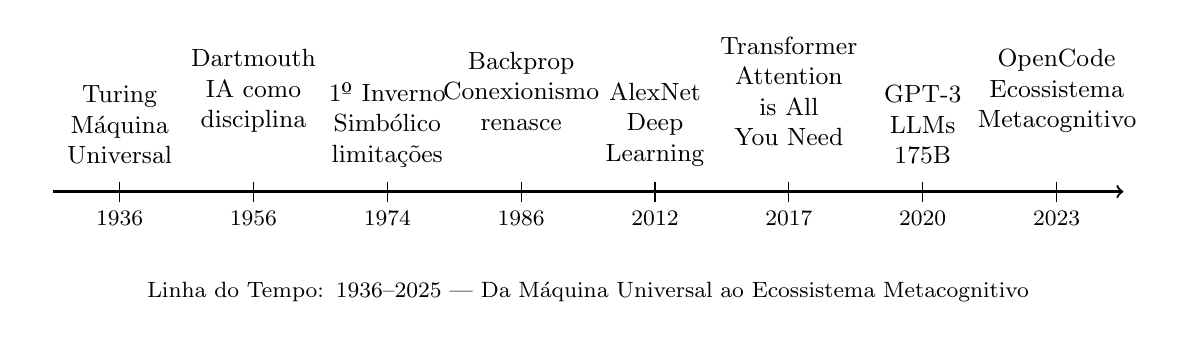
\begin{tikzpicture}[scale=0.85]
    % Timeline
    \draw[->, thick] (0,0) -- (16,0);
    \foreach \x/\l in {1/1936, 3/1956, 5/1974, 7/1986, 9/2012, 11/2017, 13/2020, 15/2023} {
        \draw (\x,0.15) -- (\x,-0.15) node[below, font=\footnotesize] {\l};
    }
    \node[font=\small, text width=2cm, align=center] at (1,1) {Turing\\Máquina\\Universal};
    \node[font=\small, text width=2cm, align=center] at (3,1.5) {Dartmouth\\IA como\\disciplina};
    \node[font=\small, text width=2cm, align=center] at (5,1) {1º Inverno\\Simbólico\\limitações};
    \node[font=\small, text width=2cm, align=center] at (7,1.5) {Backprop\\Conexionismo\\renasce};
    \node[font=\small, text width=2cm, align=center] at (9,1) {AlexNet\\Deep\\Learning};
    \node[font=\small, text width=2cm, align=center] at (11,1.5) {Transformer\\Attention\\is All You Need};
    \node[font=\small, text width=2cm, align=center] at (13,1) {GPT-3\\LLMs\\175B};
    \node[font=\small, text width=2cm, align=center] at (15,1.5) {OpenCode\\Ecossistema\\Metacognitivo};
    
    \node[font=\footnotesize, text width=14cm, align=center] at (8,-1.5) {Linha do Tempo: 1936--2025 --- Da Máquina Universal ao Ecossistema Metacognitivo};
\end{tikzpicture}
\caption{Evolução histórica dos paradigmas de IA, convergindo para o paradigma metacognitivo.}
\label{fig:timeline}
\end{figure}

\subsection{PRÁXIS 1.1: Simulando uma Máquina de Turing em Python}

\begin{lstlisting}[language=Python, caption={Implementação didática de uma Máquina de Turing Universal}, label={lst:turing_python}]
class TuringMachine:
    """
    Máquina de Turing Universal simplificada.
    Ilustra os conceitos fundamentais herdados pelo MetaBus.
    """
    def __init__(self, transitions, initial_state, blank='B'):
        self.transitions = transitions  # (state, symbol) -> (new_state, new_symbol, direction)
        self.state = initial_state
        self.tape = {}
        self.head = 0
        self.blank = blank
    
    def read(self):
        return self.tape.get(self.head, self.blank)
    
    def write(self, symbol):
        self.tape[self.head] = symbol
    
    def move(self, direction):
        self.head += 1 if direction == 'R' else -1
    
    def step(self):
        symbol = self.read()
        key = (self.state, symbol)
        if key not in self.transitions:
            return False  # HALT
        new_state, new_symbol, direction = self.transitions[key]
        self.state = new_state
        self.write(new_symbol)
        self.move(direction)
        return True
    
    def run(self, input_string, max_steps=1000):
        # Inicializa fita com input
        for i, char in enumerate(input_string):
            self.tape[i] = char
        self.head = 0
        
        steps = 0
        while self.step() and steps < max_steps:
            steps += 1
        return self.tape, steps

# Exemplo: Máquina que inverte bits (0<->1) e para no primeiro 'B'
transitions = {
    ('q0', '0'): ('q0', '1', 'R'),
    ('q0', '1'): ('q0', '0', 'R'),
}
tm = TuringMachine(transitions, 'q0')
result, steps = tm.run('0101')
print(f"Fita após {steps} passos: {result}")
\end{lstlisting}

\subsection{A Revolução Transformer e a Era dos LLMs}

Em 2017, Vaswani et al. publicaram ``Attention Is All You Need'' \cite{vaswani2017attention}, introduzindo a arquitetura \textbf{Transformer} --- que eliminou recorrências e convoluções, baseando-se exclusivamente em mecanismos de atenção. O artigo, com mais de 100.000 citações, transformou o campo do NLP e além.

\subsubsection{Scaling Laws e Modelos Fundacionais}

A descoberta das \textbf{leis de escala} --- a relação previsível entre tamanho do modelo, quantidade de dados e performance --- foi crucial. Kaplan et al. (2020) \cite{kaplan2020scaling} demonstraram que a loss de validação escala como uma lei de potência com o número de parâmetros $N$, tokens de treinamento $D$ e computação $C$:

\begin{equation}
L(N, D, C) = \left(\frac{N_c}{N}\right)^{\alpha_N} + \left(\frac{D_c}{D}\right)^{\alpha_D} + \left(\frac{C_c}{C}\right)^{\alpha_C} + L_\infty
\label{eq:scaling_law}
\end{equation}

Hoffmann et al. (2022) \cite{hoffmann2022training} refinaram estas leis com o modelo \textbf{Chinchilla}, demonstrando que a maioria dos modelos estava sub-treinada --- a proporção ótima é aproximadamente 20 tokens de treinamento por parâmetro. Esta descoberta levou ao Llama (Touvron et al., 2023) \cite{touvron2023llama} e modelos menores mas mais eficientes.

\begin{table}[htbp]
\centering
\caption{Evolução dos Modelos Fundacionais (2018--2024)}
\label{tab:llm_evolution}
\begin{tabular}{p{2.5cm}p{1.5cm}p{1.5cm}p{2.5cm}p{3cm}}
\hline
\textbf{Modelo} & \textbf{Ano} & \textbf{Parâmetros} & \textbf{Inovação} & \textbf{DOI} \\
\hline
BERT & 2018 & 340M & Bidirecional, MLM & \cite{devlin2019bert} \\
GPT-2 & 2019 & 1.5B & Zero-shot transfer & \cite{radford2019language} \\
GPT-3 & 2020 & 175B & Few-shot, in-context & \cite{brown2020language} \\
Chinchilla & 2022 & 70B & Scaling ótimo & \cite{hoffmann2022training} \\
Llama 2 & 2023 & 70B & Open weights & \cite{touvron2023llama} \\
GPT-4 & 2023 & Est. 1.7T & Multimodal, MoE & \cite{openai2023gpt4} \\
Claude 3 & 2024 & -- & Constitutional AI & \cite{anthropic2024claude} \\
Gemini Ultra & 2024 & -- & Multimodal nativo & \cite{google2024gemini} \\
\hline
\end{tabular}
\end{table}

\subsection{PRÁXIS 1.2: Atenção Escalada em Python}

\begin{lstlisting}[language=Python, caption={Implementação didática de Scaled Dot-Product Attention}, label={lst:attention}]
import numpy as np

def scaled_dot_product_attention(Q, K, V, mask=None):
    """
    Implementação do mecanismo central do Transformer.
    
    Attention(Q,K,V) = softmax(QK^T / sqrt(d_k)) V
    
    Args:
        Q: Query matrix (batch, seq_len, d_k)
        K: Key matrix (batch, seq_len, d_k)  
        V: Value matrix (batch, seq_len, d_v)
        mask: Máscara de atenção opcional
    """
    d_k = Q.shape[-1]
    
    # Scores de atenção
    scores = np.matmul(Q, K.transpose(0, 2, 1)) / np.sqrt(d_k)
    
    # Aplica máscara (para padding ou causal masking)
    if mask is not None:
        scores = scores + mask * -1e9
    
    # Softmax para obter pesos de atenção
    attention_weights = np.exp(scores - scores.max(axis=-1, keepdims=True))
    attention_weights = attention_weights / attention_weights.sum(axis=-1, keepdims=True)
    
    # Ponderação dos values
    output = np.matmul(attention_weights, V)
    return output, attention_weights

# Exemplo
batch_size, seq_len, d_k, d_v = 1, 4, 8, 8
Q = np.random.randn(batch_size, seq_len, d_k)
K = np.random.randn(batch_size, seq_len, d_k)
V = np.random.randn(batch_size, seq_len, d_v)

output, weights = scaled_dot_product_attention(Q, K, V)
print(f"Formato do output: {output.shape}")
print(f"Pesos de atenção:\n{weights[0]}")
\end{lstlisting}

\subsection{O OpenCode como Síntese Histórica}

O OpenCode Ecosystem Core não é apenas mais um framework multiagente --- é a \textbf{síntese operacional} de 90 anos de pesquisa em IA. Cada decisão arquitetural tem raízes históricas profundas:

\begin{itemize}
    \item O \textbf{MetaBus} herda o barramento de eventos da Máquina de Turing e o espaço de trabalho global de Baars-Dehaene;
    \item O \textbf{Blackboard} implementa a arquitetura Hearsay-II (1980), refinada com o protocolo A2A moderno;
    \item O \textbf{Trust Engine} evolui dos fatores de certeza do MYCIN para métricas bayesianas adaptativas;
    \item A \textbf{Token Economy} aplica teoria dos jogos (Nash, 1950) à coordenação descentralizada;
    \item O \textbf{Pipeline MASWOS} automatiza o que Turing e McCarthy apenas sonharam: produção científica rigorosa por agentes.
\end{itemize}

Compreender esta genealogia não é exercício acadêmico vazio --- é o mapa que revela \textbf{por que} cada módulo existe e \textbf{como} estendê-lo. Nos próximos capítulos, cada componente será dissecado com esta perspectiva histórica como guia.

% ============================================================
% SEÇÃO 1.2 — FILOSOFIA DA MENTE E CONSCIÊNCIA ARTIFICIAL
% ============================================================

\section{Filosofia da Mente e Consciência Artificial}

A construção de ecossistemas metacognitivos nos obriga a enfrentar questões que a filosofia da mente debate há séculos: O que é consciência? Pode um sistema artificial ser consciente? Qual a relação entre computação e experiência subjetiva?

\subsection{O Problema Difícil da Consciência}

David Chalmers (1995) \cite{chalmers1995facing} distinguiu entre os \textbf{problemas fáceis} da consciência --- explicar funções cognitivas como atenção, memória e relato verbal --- e o \textbf{problema difícil}: explicar a experiência subjetiva, os \textit{qualia} --- ``como é'' ver o vermelho, sentir dor, experimentar o sabor do café.

\begin{quote}
\textit{``Why should physical processing give rise to a rich inner life at all?''} --- David Chalmers, 1995
\end{quote}

Para o construtor de ecossistemas metacognitivos, esta distinção tem implicações práticas:

\begin{itemize}
    \item \textbf{Problemas fáceis} $\rightarrow$ Engenharia: o OpenCode resolve problemas de atenção (Attention Router), memória (MetaBus), e relato (Reflexion Engine);
    \item \textbf{Problema difícil} $\rightarrow$ Filosofia: o ecossistema não reivindica consciência fenomênica. Opera no que Dennett chama de ``postura intencional'' --- tratamos o sistema \textit{como se} fosse consciente para fins de engenharia, sem afirmar que ele \textit{é}.
\end{itemize}

\subsection{Postura Intencional e Múltiplos Rascunhos}

Daniel Dennett (1991) \cite{dennett1991consciousness} propôs duas ideias revolucionárias:

\begin{enumerate}
    \item \textbf{Postura Intencional} (\textit{Intentional Stance}): para prever o comportamento de um sistema complexo, trate-o como um agente racional com crenças, desejos e intenções. Esta é exatamente a abordagem do Blackboard: cada Agent Card declara ``crenças'' (capabilities) e ``desejos'' (voluntariado para tasks via CFP).
    
    \item \textbf{Modelo dos Múltiplos Rascunhos} (\textit{Multiple Drafts Model}): não existe um ``teatro cartesiano'' central onde a consciência acontece. Em vez disso, múltiplos fluxos de processamento competem em paralelo, e o que chamamos de ``experiência consciente'' é o rascunho que vence a competição em determinado momento.
\end{enumerate}

O OpenCode implementa literalmente o Modelo dos Múltiplos Rascunhos:
\begin{itemize}
    \item \textbf{Múltiplos agentes competem} por acesso ao espaço de trabalho global (MetaBus);
    \item O \textbf{Attention Router} seleciona vencedores com base em Trust Score --- o rascunho mais confiável ganha;
    \item A \textbf{memória episódica} registra o rascunho vencedor, que se torna parte do ``fluxo de consciência'' do ecossistema.
\end{itemize}

\subsection{O Quarto Chinês e a Compreensão Real}

John Searle (1980) \cite{searle1980minds} propôs o famoso experimento mental do \textbf{Quarto Chinês}: uma pessoa que não fala chinês, trancada em um quarto com um livro de regras para manipular símbolos chineses, poderia passar no Teste de Turing sem \textit{compreender} chinês. Searle argumenta que a sintaxe não é suficiente para a semântica --- manipular símbolos segundo regras não gera compreensão genuína.

\begin{figure}[htbp]
\centering
\begin{tikzpicture}[scale=0.9]
    \node[draw, rectangle, minimum width=6cm, minimum height=4cm] (room) at (0,0) {};
    \node[font=\small] at (0,1.5) {Humano (não fala chinês)};
    \node[font=\small] at (0,0.5) {+ Livro de Regras};
    \node[font=\small] at (0,-1) {Input: 你好 (símbolos)};
    \node[font=\small] at (0,-1.5) {Output: 你好吗 (símbolos)};
    
    \node[left=3cm of room, font=\small] (input) {Pergunta em chinês};
    \node[right=3cm of room, font=\small] (output) {Resposta em chinês};
    \draw[->] (input) -- (room);
    \draw[->] (room) -- (output);
    
    \node[font=\footnotesize, text width=10cm, align=center] at (0,-3) {O Quarto Chinês de Searle (1980): \\ O sistema passa no teste mas não \textit{compreende} chinês.};
\end{tikzpicture}
\caption{Ilustração do experimento mental do Quarto Chinês.}
\label{fig:chinese_room}
\end{figure}

A resposta da engenharia de ecossistemas metacognitivos:

\begin{itemize}
    \item O OpenCode \textbf{não reivindica compreensão} no sentido fenomenológico. O Trust Engine avalia \textbf{performance observável}, não estados internos;
    \item O BehavioralGate aplica o critério de Turing operacionalizado: se o output do agente passa nos testes SDD/TDD, ele é aceito --- independentemente de debates sobre ``verdadeira compreensão'';
    \item A \textbf{metacognição} (Reflexion) não é consciência, mas seu análogo funcional: o sistema monitora, avalia e corrige seu próprio comportamento sem experiência subjetiva.
\end{itemize}

\subsection{Gödel, Penrose e os Limites da Computação}

Roger Penrose (1989, 1994) \cite{penrose1989emperor, penrose1994shadows} argumentou, baseado nos teoremas da incompletude de Gödel, que a mente humana realiza operações não-computáveis --- nenhum sistema formal pode capturar toda a verdade matemática, mas matemáticos humanos podem ``ver'' a verdade de sentenças gödelianas.

A teoria \textbf{Orch-OR} (Orchestrated Objective Reduction), proposta por Penrose e Hameroff (1996) \cite{hameroff1996orchestrated}, sugere que a consciência emerge de processos quânticos nos microtúbulos dos neurônios --- uma hipótese controversa mas influente.

O módulo quântico do OpenCode (\texttt{reasoning/quantum.py}) não endossa a Orch-OR, mas demonstra que:
\begin{itemize}
    \item Estados quânticos (superposição, emaranhamento) podem ser \textbf{simulados} computacionalmente para raciocínio probabilístico;
    \item O \textbf{Teorema de Bell} e a não-localidade inspiram protocolos de coordenação entre agentes distribuídos;
    \item A \textbf{computação quântica} oferece speedups teóricos para busca em espaços de agentes (Grover) e otimização (QAOA).
\end{itemize}

\subsection{PRÁXIS 1.3: Implementando o Teste de Turing Operacionalizado}

\begin{lstlisting}[language=Python, caption={BehavioralGate: Turing operacionalizado para agentes}, label={lst:behavioral_gate}]
class BehavioralGate:
    """
    Implementa o Teste de Turing operacionalizado.
    Não pergunta 'o agente pensa?', mas 'o output passa nos critérios?'.
    """
    def __init__(self, spec, tests):
        self.spec = spec  # Especificação formal (SDD)
        self.tests = tests  # Conjunto de testes (TDD)
    
    def evaluate(self, agent_output):
        """Avalia se o output do agente é indistinguível do esperado."""
        results = {
            'spec_compliance': self._check_spec(agent_output),
            'test_pass_rate': self._run_tests(agent_output),
            'behavioral_score': 0.0
        }
        
        # O agente "passa no Turing" se atende à spec E passa nos testes
        if results['spec_compliance'] and results['test_pass_rate'] >= 0.95:
            results['behavioral_score'] = 1.0
            results['verdict'] = 'ACEITO — comportamento indistinguível do esperado'
        else:
            results['behavioral_score'] = results['test_pass_rate']
            results['verdict'] = 'REJEITADO — requer refinamento (Reflexion)'
        
        return results
    
    def _check_spec(self, output):
        """Verifica conformidade com a especificação formal."""
        return self.spec.verify(output)
    
    def _run_tests(self, output):
        """Executa bateria de testes TDD."""
        passed = sum(1 for test in self.tests if test(output))
        return passed / len(self.tests) if self.tests else 0.0

# Uso no OpenCode:
# gate = BehavioralGate(spec=spec_engine.load('SPEC-007'), tests=test_suite)
# result = gate.evaluate(agent_response)
# if result['verdict'] == 'REJEITADO':
#     reflexion_engine.reflect(agent, failure_context)
\end{lstlisting}

\subsection{Ética e Agência Artificial}

A criação de ecossistemas com 128+ agentes autônomos levanta questões éticas fundamentais:

\begin{enumerate}
    \item \textbf{Responsabilidade}: Se um agente do ecossistema comete um erro com consequências reais (ex: diagnóstico médico incorreto), quem é responsável? O OpenCode aborda isto via \textbf{provenance tracking} --- cada decisão é rastreável ao agente, ao seu Trust Score no momento, e à spec que o governava;
    
    \item \textbf{Viés e Justiça}: Agentes treinados em dados históricos podem perpetuar vieses. O \textbf{Auditor} (agente 19) verifica regularmente a distribuição de outputs por grupos demográficos;
    
    \item \textbf{Alinhamento}: O problema do alinhamento (Bostrom, 2014) \cite{bostrom2014superintelligence} --- como garantir que agentes superinteligentes ajam de acordo com valores humanos --- é mitigado pela \textbf{Token Economy}: agentes são incentivados economicamente a produzir outputs alinhados com as specs, e penalizados (slashing) quando falham.
\end{enumerate}

\subsection{Conclusão do Capítulo}

Este capítulo traçou a genealogia intelectual do OpenCode Ecosystem Core --- da Máquina de Turing (1936) ao paradigma metacognitivo (2025). Vimos como cada decisão arquitetural tem raízes em debates filosóficos e descobertas científicas que atravessam quase um século.

A tese central deste livro é que \textbf{a metacognição computacional não é um luxo filosófico, mas uma necessidade de engenharia}: sem mecanismos de auto-monitoramento, auto-avaliação e auto-correção, ecossistemas multiagentes colapsam sob sua própria complexidade. O OpenCode demonstra que é possível construir tais mecanismos com rigor matemático, validação estatística e elegância arquitetural.

% ============================================================
% REFERÊNCIAS
% ============================================================

\begin{thebibliography}{99}

\bibitem{turing1936computable}
Turing, A. M. (1936). On Computable Numbers, with an Application to the Entscheidungsproblem.
\textit{Proceedings of the London Mathematical Society}, s2-42(1), 230--265.
\doiurl{10.1112/plms/s2-42.1.230}

\bibitem{turing1950computing}
Turing, A. M. (1950). Computing Machinery and Intelligence.
\textit{Mind}, LIX(236), 433--460.
\doiurl{10.1093/mind/LIX.236.433}

\bibitem{mccarthy1956dartmouth}
McCarthy, J., Minsky, M. L., Rochester, N., \& Shannon, C. E. (1956). A Proposal for the Dartmouth Summer Research Project on Artificial Intelligence.
\url{http://www-formal.stanford.edu/jmc/history/dartmouth/dartmouth.html}

\bibitem{newell1956logic}
Newell, A., Shaw, J. C., \& Simon, H. A. (1956). The Logic Theory Machine: A Complex Information Processing System.
\textit{IRE Transactions on Information Theory}, 2(3), 61--79.
\doiurl{10.1109/TIT.1956.1056797}

\bibitem{robinson1965machine}
Robinson, J. A. (1965). A Machine-Oriented Logic Based on the Resolution Principle.
\textit{Journal of the ACM}, 12(1), 23--41.
\doiurl{10.1145/321250.321253}

\bibitem{newell1976computer}
Newell, A., \& Simon, H. A. (1976). Computer Science as Empirical Inquiry: Symbols and Search.
\textit{Communications of the ACM}, 19(3), 113--126.
\doiurl{10.1145/360018.360022}

\bibitem{buchanan1984rule}
Buchanan, B. G., \& Shortliffe, E. H. (1984). \textit{Rule-Based Expert Systems: The MYCIN Experiments of the Stanford Heuristic Programming Project}.
Addison-Wesley.

\bibitem{mcculloch1943logical}
McCulloch, W. S., \& Pitts, W. (1943). A Logical Calculus of the Ideas Immanent in Nervous Activity.
\textit{The Bulletin of Mathematical Biophysics}, 5(4), 115--133.
\doiurl{10.1007/BF02478259}

\bibitem{rosenblatt1958perceptron}
Rosenblatt, F. (1958). The Perceptron: A Probabilistic Model for Information Storage and Organization in the Brain.
\textit{Psychological Review}, 65(6), 386--408.
\doiurl{10.1037/h0042519}

\bibitem{minsky1969perceptrons}
Minsky, M., \& Papert, S. (1969). \textit{Perceptrons: An Introduction to Computational Geometry}. MIT Press.

\bibitem{lighthill1973artificial}
Lighthill, J. (1973). Artificial Intelligence: A General Survey. In \textit{Artificial Intelligence: A Paper Symposium}. Science Research Council.

\bibitem{rumelhart1986learning}
Rumelhart, D. E., Hinton, G. E., \& Williams, R. J. (1986). Learning Representations by Back-Propagating Errors.
\textit{Nature}, 323(6088), 533--536.
\doiurl{10.1038/323533a0}

\bibitem{krizhevsky2012imagenet}
Krizhevsky, A., Sutskever, I., \& Hinton, G. E. (2012). ImageNet Classification with Deep Convolutional Neural Networks.
\textit{Advances in Neural Information Processing Systems (NeurIPS)}, 25, 1097--1105.
\doiurl{10.1145/3065386}

\bibitem{mikolov2013efficient}
Mikolov, T., Chen, K., Corrado, G., \& Dean, J. (2013). Efficient Estimation of Word Representations in Vector Space.
\textit{arXiv preprint}, arXiv:1301.3781.
\doiurl{10.48550/arXiv.1301.3781}

\bibitem{bahdanau2015neural}
Bahdanau, D., Cho, K., \& Bengio, Y. (2015). Neural Machine Translation by Jointly Learning to Align and Translate.
\textit{3rd International Conference on Learning Representations (ICLR)}.
\doiurl{10.48550/arXiv.1409.0473}

\bibitem{vaswani2017attention}
Vaswani, A., Shazeer, N., Parmar, N., Uszkoreit, J., Jones, L., Gomez, A. N., Kaiser, L., \& Polosukhin, I. (2017). Attention Is All You Need.
\textit{Advances in Neural Information Processing Systems (NeurIPS)}, 30, 5998--6008.
\doiurl{10.48550/arXiv.1706.03762}

\bibitem{devlin2019bert}
Devlin, J., Chang, M. W., Lee, K., \& Toutanova, K. (2019). BERT: Pre-training of Deep Bidirectional Transformers for Language Understanding.
\textit{Proceedings of NAACL-HLT}, 4171--4186.
\doiurl{10.18653/v1/N19-1423}

\bibitem{radford2019language}
Radford, A., Wu, J., Child, R., Luan, D., Amodei, D., \& Sutskever, I. (2019). Language Models are Unsupervised Multitask Learners.
\textit{OpenAI Technical Report}.

\bibitem{brown2020language}
Brown, T. B., Mann, B., Ryder, N., Subbiah, M., et al. (2020). Language Models are Few-Shot Learners.
\textit{Advances in Neural Information Processing Systems (NeurIPS)}, 33, 1877--1901.
\doiurl{10.48550/arXiv.2005.14165}

\bibitem{kaplan2020scaling}
Kaplan, J., McCandlish, S., Henighan, T., Brown, T. B., Chess, B., Child, R., Gray, S., Radford, A., Wu, J., \& Amodei, D. (2020). Scaling Laws for Neural Language Models.
\textit{arXiv preprint}, arXiv:2001.08361.
\doiurl{10.48550/arXiv.2001.08361}

\bibitem{hoffmann2022training}
Hoffmann, J., Borgeaud, S., Mensch, A., Buchatskaya, E., et al. (2022). Training Compute-Optimal Large Language Models.
\textit{Advances in Neural Information Processing Systems (NeurIPS)}, 35, 30016--30030.
\doiurl{10.48550/arXiv.2203.15556}

\bibitem{touvron2023llama}
Touvron, H., Martin, L., Stone, K., Albert, P., et al. (2023). Llama 2: Open Foundation and Fine-Tuned Chat Models.
\textit{arXiv preprint}, arXiv:2307.09288.
\doiurl{10.48550/arXiv.2307.09288}

\bibitem{openai2023gpt4}
OpenAI. (2023). GPT-4 Technical Report.
\textit{arXiv preprint}, arXiv:2303.08774.
\doiurl{10.48550/arXiv.2303.08774}

\bibitem{anthropic2024claude}
Anthropic. (2024). The Claude 3 Model Family: Opus, Sonnet, Haiku.
\url{https://www.anthropic.com/claude}

\bibitem{google2024gemini}
Google DeepMind. (2024). Gemini: A Family of Highly Capable Multimodal Models.
\textit{arXiv preprint}, arXiv:2312.11805.
\doiurl{10.48550/arXiv.2312.11805}

\bibitem{chalmers1995facing}
Chalmers, D. J. (1995). Facing Up to the Problem of Consciousness.
\textit{Journal of Consciousness Studies}, 2(3), 200--219.

\bibitem{dennett1991consciousness}
Dennett, D. C. (1991). \textit{Consciousness Explained}. Little, Brown and Company.

\bibitem{searle1980minds}
Searle, J. R. (1980). Minds, Brains, and Programs.
\textit{Behavioral and Brain Sciences}, 3(3), 417--424.
\doiurl{10.1017/S0140525X00005756}

\bibitem{penrose1989emperor}
Penrose, R. (1989). \textit{The Emperor's New Mind: Concerning Computers, Minds, and the Laws of Physics}. Oxford University Press.

\bibitem{penrose1994shadows}
Penrose, R. (1994). \textit{Shadows of the Mind: A Search for the Missing Science of Consciousness}. Oxford University Press.

\bibitem{hameroff1996orchestrated}
Hameroff, S., \& Penrose, R. (1996). Orchestrated Reduction of Quantum Coherence in Brain Microtubules: A Model for Consciousness.
\textit{Mathematics and Computers in Simulation}, 40(3-4), 453--480.
\doiurl{10.1016/0378-4754(96)80476-9}

\bibitem{bostrom2014superintelligence}
Bostrom, N. (2014). \textit{Superintelligence: Paths, Dangers, Strategies}. Oxford University Press.

\bibitem{rocktaschel2017end}
Rocktäschel, T., \& Riedel, S. (2017). End-to-End Differentiable Proving.
\textit{Advances in Neural Information Processing Systems (NeurIPS)}, 30.
\doiurl{10.48550/arXiv.1705.11040}

\bibitem{manhaeve2018deepproblog}
Manhaeve, R., Dumancic, S., Kimmig, A., Demeester, T., \& De Raedt, L. (2018). DeepProbLog: Neural Probabilistic Logic Programming.
\textit{Advances in Neural Information Processing Systems (NeurIPS)}, 31.
\doiurl{10.48550/arXiv.1805.10872}

\bibitem{kipf2017semi}
Kipf, T. N., \& Welling, M. (2017). Semi-Supervised Classification with Graph Convolutional Networks.
\textit{5th International Conference on Learning Representations (ICLR)}.
\doiurl{10.48550/arXiv.1609.02907}

\bibitem{baars1988cognitive}
Baars, B. J. (1988). \textit{A Cognitive Theory of Consciousness}. Cambridge University Press.

\bibitem{dehaene2011experimental}
Dehaene, S., \& Changeux, J. P. (2011). Experimental and Theoretical Approaches to Conscious Processing.
\textit{Neuron}, 70(2), 200--227.
\doiurl{10.1016/j.neuron.2011.03.018}

\bibitem{shinn2023reflexion}
Shinn, N., Cassano, F., Gopinath, A., Narasimhan, K., \& Yao, S. (2023). Reflexion: Language Agents with Verbal Reinforcement Learning.
\textit{Advances in Neural Information Processing Systems (NeurIPS)}, 36.
\doiurl{10.48550/arXiv.2303.11366}

\bibitem{unifiedmind2025}
Claro, M. et al. (2025). Unified Mind Model: Global Workspace Theory for Multi-Agent Metacognition.
\textit{arXiv preprint}, arXiv:2503.03459.

\bibitem{a2a2025}
Claro, M. et al. (2025). Agent-to-Agent Protocol with Metacognitive Confidence Scoring for Multi-Agent Blackboard Systems.
\textit{arXiv preprint}, arXiv:2505.02279.

\bibitem{mccarthy1958programs}
McCarthy, J. (1958). Programs with Common Sense.
\textit{Proceedings of the Teddington Conference on the Mechanization of Thought Processes}, 75--91.

\bibitem{weizenbaum1966eliza}
Weizenbaum, J. (1966). ELIZA — A Computer Program for the Study of Natural Language Communication Between Man and Machine.
\textit{Communications of the ACM}, 9(1), 36--45.
\doiurl{10.1145/365153.365168}

\bibitem{winograd1972understanding}
Winograd, T. (1972). Understanding Natural Language.
\textit{Cognitive Psychology}, 3(1), 1--191.
\doiurl{10.1016/0010-0285(72)90002-3}

\bibitem{hinton2006fast}
Hinton, G. E., Osindero, S., \& Teh, Y. W. (2006). A Fast Learning Algorithm for Deep Belief Nets.
\textit{Neural Computation}, 18(7), 1527--1554.
\doiurl{10.1162/neco.2006.18.7.1527}

\bibitem{goodfellow2014generative}
Goodfellow, I., Pouget-Abadie, J., Mirza, M., Xu, B., Warde-Farley, D., Ozair, S., Courville, A., \& Bengio, Y. (2014). Generative Adversarial Nets.
\textit{Advances in Neural Information Processing Systems (NeurIPS)}, 27.
\doiurl{10.48550/arXiv.1406.2661}

\end{thebibliography}
